%%%%%%%%%%%%%%%%%
% elastic

\section{Elastické systémy}
\label{sec:elastic}
Elastické systémy slouží k simulaci těles jako je látka, tkanina, lana, ale i rosol.
Elastický objekt mění svůj tvar v průběhu času.
Proto je výpočet jeho pohybu odlišný od výpočtu dynamiky tuhého tělesa.
Pohyb tuhého tělesa si můžeme rozložit na posuvnou rychlost a rotační rychlost.
Pokud na takové těleso působíme silou, jsou body tělesa přímo ovlivňovány.
Elastické těleso je složeno z bodů a vazeb, přičemž každý bod má vlastní výpočet dynamiky.
Pokud tedy na elastické těleso působíme silou, účinky síly jsou postupně distribuovány pomocí vazeb do bodů.

Elastický systém si můžeme představit jako speciální obdobu částicového systému.
Částice (uzly) představují vrcholy objektu, vrcholy trojúhelníků.
Každá částice má svoji hmotnost, pozici a rychlost.
Oproti částicovým systémům obsahuje částice i seznam vazeb, které ovlivňují její pohyb.
Vazba je spoj mezi dvěma částicemi.
Nese informaci o své počáteční délce a své tuhosti.
Dále obsahuje informaci, které dva uzly spojuje.
Elastický systém je tedy složen ze dvou základních druhů elementů: uzlů a spojů.

Pohyb elastického systému si popíšeme diferenciálními rovnicemi.
Každá částice má svoji pozici $p$ a rychlost $v$.
Pro výpočet nové pozice $p(t+dt)$ potřebujeme rychlost $v(t)$ a krok času $dt$.
Pro výpočet nové rychlosti $v(t+dt)$ potřebujeme zrychlení $a(t)$ a krok času $dt$.
Diferenciální rovnice pro výpočet pozice:
\begin{equation}
\label{eq:pozice0}
\frac{\partial p}{\partial t} = v
\end{equation}
Rovnici \ref{eq:pozice0} zintegrujeme a dostaneme tvar:
\begin{equation}
\label{eq:pozice1}
p(t)=p(0)+\int_0^t v(t) dt
\end{equation}
V rovnici \ref{eq:pozice1} je $p(0)$ počáteční pozice částice v čase $t=0$.
$p(t)$ respektive $v(t)$ je pozice respektive rychlost v čase $t$.
Rovnici \ref{eq:pozice1} si můžeme vyjádřit schématem s integrátorem na obrázku \ref{fig:intpos}.
\begin{figure}[h]
\centering
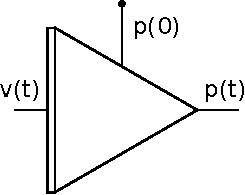
\includegraphics[height=3cm,keepaspectratio]{obr/intpos.pdf}
\caption{Integrátor reprezentující rovnici \ref{eq:pozice1}}
\label{fig:intpos}
\end{figure}
Diferenciální rovnice pro výpočet rychlosti:
\begin{equation}
\label{eq:rychlost0}
\frac{\partial v}{\partial t} = a
\end{equation}
Rovnici \ref{eq:rychlost0} zintegrujeme a výsledný tvar je:
\begin{equation}
\label{eq:rychlost1}
v(t)=v(0)+\int_0^t a(t) dt
\end{equation}
$a(t)$ v rovnici \ref{eq:rychlost1} reprezentuje zrychlení, $v(0)$ počáteční rychlost a $v(t)$ rychlost v čase $t$.
Schéma pro rovnici \ref{eq:rychlost1} je obdobné schématu \ref{fig:intpos}.
Schémata můžeme spojit v jedno, které je znázorněné na obrázku \ref{fig:intvelpos}
\begin{figure}[h]
\centering
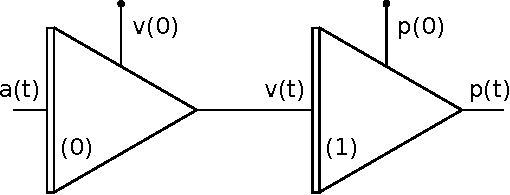
\includegraphics[height=3cm,keepaspectratio]{obr/intvelpos.pdf}
\caption{Schéma představující spojení rovnic \ref{eq:pozice1} a \ref{eq:rychlost1}}
\label{fig:intvelpos}
\end{figure}
Jelikož vytváříme elastický systém v trojrozměrném prostoru je zrychlení, rychlost a pozice třísložkový vektor.
Schéma \ref{fig:intvelpos} nám již dokáže vypočítat pozici jedné částice v čase $t$.
Zbývá zjisti zrychlení, tedy vstup integrátoru $(0)$.
Zrychlení částice se odvíjí od druhého Newtonova zákonu o působení síly na hmotné těleso:
\begin{equation}
\label{eq:newton}
a=\frac{1}{m} \cdot F
\end{equation}
Nyní již víme, jak se částice (uzel elastického systému) zachová, pokud na ni zapůsobíme silou.
Síla je složena z gravitační síly $F_g=m \cdot g$, která je pro daný uzel konstantní a síly vyvolané spoji daného uzlu.
Spoj mezi dvěma uzly si můžeme představit jako pružinu.
Sílu, kterou pružina působí na dva uzly si vyjádříme vztahem:
\begin{equation}
\label{eq:pruzina}
F=-k \cdot x
\end{equation}
Ve vztahu \ref{eq:pruzina} je $k$ tuhost pružiny (nebo spoje) a $x=l_0-l$ je výchylka pružiny z rovnovážného stavu.
$l_0$ je počáteční délka spoje a $l$ je aktuální délka spoje v čase $t$.
Absolutní velikost síly vyvolané spoji na uzel $i$ je:
\begin{equation}
\label{eq:sumpruz}
|F_i|=\sum_{j=1}^n -k_{i,j} \cdot ({l_0}_{i,j}-|p_i p_j|) \cdot s_{i,j}
\end{equation}
$n$ je počet uzlů.
${l_0}_{i,j}$ je počáteční délka spoje mezi uzly $i,j$.
$p_i,p_j$ jsou pozice uzlů a $s_{i,j}=1$ pokud je mezi uzly $i,j$ spoj.
Jinak je $s_{i,j}=0$.
Stejně jako pro pozici a rychlost, je i síla třísložkový vektor.
Označme $e_{i,j}=(p_j-p_i)/|p_i p_j|$ normalizovaný vektor spoje z uzlu $i$ do $j$.
Výsledná síla působící na uzel $i$ je:
\begin{equation}
\label{eq:sumpruz1}
F_i=\sum_{j=1}^n -k_{i,j} \cdot ({l_0}_{i,j}-|p_i p_j|) \cdot s_{i,j} \cdot e_{i,j} =
\sum_{j=1}^n -s_{i,j} \cdot k_{i,j} \left( \frac{{l_0}_{i,j}}{|p_i p_j|}-1 \right) (p_j-p_i)
\end{equation}
Nyní již známe vše, abychom mohli vytvořit schéma obecného elastického systému.
Schéma je znázorněné na obrázku \ref{fig:intschema}
\begin{figure}[h]
\centering
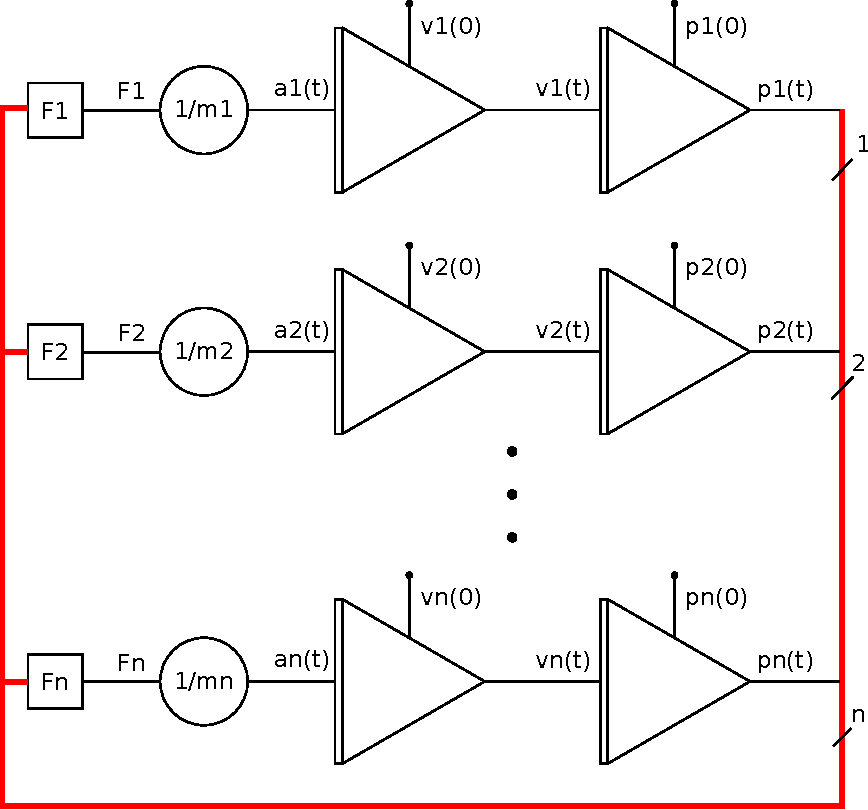
\includegraphics[height=10cm,keepaspectratio]{obr/intschema.pdf}
\caption{Schéma obecného elastického systému.
Jednotky $F_1 - F_n$ počítají sílu podle vztahu \ref{eq:sumpruz1}}
\label{fig:intschema}
\end{figure}

Diferenciální rovnice musíme vyřešit pomocí numerických metod.
Existuje několik druhů numerických metod.
Nejznámější je Eulerova metoda.
Přesnost numerických metod závisí na velikosti kroku času $dt$ a stupně metody.

\subsection{Eulerova metoda}
Eulerova metoda je jednoduchá numerická metoda pro řešení diferenciálních rovnic.
Je dána vztahem:
%$$y'(t) \approx \frac{y(t+dt)-y(t)}{dt} $$
%$$y_0 = y(0)$$
%$$y_{n+1}=y_n+dt \cdot f(t_n,y_n)$$
\begin{eqnarray*}
\label{eq:eulerint}
y_0     &=& y(0)    \\
y_{n+1} &=& y_{n} + dt \cdot f(t_n,y_{n})
\end{eqnarray*}
$f(t_n,y_n)$ je aproximace derivace $y'_n$.
V našem případě je to vstup integrátorů ve schématu \ref{fig:intschema}.
Eulerova metoda je rychlá na výpočet a jednoduchá na implementaci.
Proto může být vhodná pro intra.
Její nevýhodou je malá přesnost.
Proto je nutné volit menší krok času než u jiných metod.
\subsection{Runge Kutta metoda}
Runge Kutta metoda čtvrtého stupně je dána vztahem:
\begin{eqnarray*}
\label{eq:rungeint}
y_0     &=& y(0)    \\
y_{n+1} &=& y_{n} + \frac{1}{6}(k_1 + 2k_2 + 2k_3 + k_4) \\
k_1     &=& dt f(t_n,y_n) \\
k_2     &=& dt f(t_n+dt/2,y_n+k_1/2) \\
k_3     &=& dt f(t_n+dt/2,y_n+k_2/2) \\
k_4     &=& dt f(t_n+dt,y_n+k_3)
\end{eqnarray*}
Runge Kutta metoda je obecně přesnější než Eulerova metoda.
Je ale výpočetně náročnější.
Pro výpočet následující hodnoty integrátoru je zapotřebí čtyřikrát vyčíslit jeho vstup.

\subsection{Stabilita numerických metod}
Numerické metody nemusí být stabilní.
Pro některé rovnice se rozkmitají.
Náš elastický systém se pro nevhodně zvolené koeficienty rozkmitá a následně rozpadne.
Musíme správně zvolit koeficienty tuhosti spojů a hmotnosti uzlů.
Velký vliv na stabilitu má krok času $dt$.
Elastický systém je tuhý systém, pokud jsou hmotnosti uzlů malé nebo pokud jsou tuhosti spojů velké.
Tato skutečnost vyplývá z rovnic \ref{eq:newton} a \ref{eq:pruzina}.
Pokud obě rovnice spojíme získáme koeficient $c=k/m$, kde $k$ je tuhost spoje a $m$ hmotnost uzlu.
Tento koeficient přibližně popisuje zesílení zpětné vazby vyznačené červenou barvou v obrázku \ref{fig:intschema}.

V programu jsem nejprve naimplementoval Eulerovu numerickou metodu.
Její největší nevýhoda byla nestabilita.
Pokud jsem v průběhu animace zvyšoval tuhosti spojů, v jednom okamžiku se elastický systém choval dle očekávání.
Pokud ale tuhost přerostla určitý práh, systém se velice rychle rozkmital a rozpadl a animaci jsem musel pusti znovu.
Proto jsem se rozhodl zkusit implemetovat Runge Kutta čtvrtého řádu.
U Runge Kutta metody elastický systém reaguje na nevhodně zvolené tuhosti a hmotnosti pomaleji.
Proto je možné se ještě z rozkmitaného stavu vrátit zpět.
Testoval jsem také rychlost.
Věděl jsem, že u Runge Kutta metody potřebuji vyčíslit čtyři koeficienty.
Výpočet jednoho kroku je tak přibližně čtyřikrát náročnější než u metody Eulerovy.
Experimentálně jsem si srovnal výsledky pro stejný elastický systém s Eulerovou metodou pro krok $dt$ a Runge Kutta metodou pro krok $4dt$.
Sledoval jsem, při jakém nastavení tuhosti spojů se systém rozkmitá.
Výsledky pro metodu Runge Kutta byly mírně lepší než pro Eulerovu metodu, proto jsem se rozhodl jej ve výsledné aplikaci využívat.
Také velmi záleželo na tvaru elastického systému.






